% Chapter Template

\chapter{Analysis and Discussion} % Main chapter title

\label{AnalysisAndDiscussion}

\lhead{Chapter \ref{AnalysisAndDiscussion}. \emph{Analysis and Discussion}}

In this chapter we will analyse different parts of the system to see if we can judge their appropriateness in solving the
problems tied to our research question.
We will first compare the mapping algorithms to see if one of them performs better then the other.
We will also look into the questions of wether we were able to generate metadata of equal or better quality than that
which is already available, and if we can add this metadata without changing the way the webpage is displayed.
We will also look at the usage data we have gotten at this point and see how it corresponds with the expected use of the system.

\section{Comparing the algorithms}
\label{ComparingAlgorithms}
To compare the two algorithms we generated a list of english nouns
which we sent through the lexitags server to get synsets that corresponded to the meanings of each word.
Both these lists were preprocessed to remove duplicates and to format them as javascript objects
\footnote{\url{https://github.com/EivindEE/Madame/tree/master/testing}}.
The final list of synsets contained 4350 unique synsets.
We wrote a short script that we used to run the synsets through the best fit algorithms,
and write a report of the results.
For the schema.org version of the test we wrote the average depth of the mapped type,
as well as the total number of times the two algorithms had the same and different mappings.
The debth was calculated as the distance from the root node in the tree,
i.e. schema:Thing it self had a depth of 0,
schema:Person which inherits directly from schema:Thing has a depth of 1 and so on.
For the SUMO version the depth of each type was unavailable,
so we only have numbers showing the agreement between the algorithms.
The full results from the tests can be found at the URL \url{https://github.com/EivindEE/Master-thesis/tree/master/AlgComparison}.

As one can read from the numbers it table \ref{table:AlgorithmResults} the results from the SUMO test
display no difference between the two algorithms when mapping from WordNet to SUMO.
The two algorithms return identical mappings in 100\% of the test cases.
This indicates that there must have beena mapping either directly from the synset,
or from the direct hypernym of the synset for each of the 4350 synsets in our test.
This makes it hard to say anything relevant about the algoritms from these results.

\begin{table}[ht] %%%% Should I change the results so that the no results found are ignored?
	\centering
	\begin{tabular}{lll}
										& Schema.org	& SUMO			\\
		Total number of synsets tested 	& 4350			& 4350			\\
		Number of identical mappings 	& 3262 (75\%)	& 4350 (100\%)	\\
		Number  of different mappings	& 1088 (25\%)	& 0	(0\%)		\\
		No result found					& 598  (13.7\%)	& 0	(0\%)
	\end{tabular}
	\caption{The testing results}
	\label{table:AlgorithmResults}
\end{table}

The schema.org results are more interesting.
The two algorithms still perform fairly equally.
Reading from table \ref{table:AlgorithmResults} we can see that the algorithms are equal in 75\% of the cases,
but we can examine the 25\% that are different and see which perform better in those cases.
We can also see that the algorithms were unable to find a mapping in 13.7\% of the cases.
These cases can't tell us much about which algorithm we should prefere,
but could be a good starting point for finding parts of the WordNet to schema.org mapping which could be enhanced.

Our predictions beforhand was that the hypernyms first approach would have fewer incorrect mappings,
but would give results at a more shallow depth.
The last prediction was the easiest to test, as we know the schema.org hierarchy and can calculate the depth of each type.
For each mapping we registered the depth of the type in the schema.org hierarchy.
These depths were averaged over the total number of mappings made.

As seen in table \ref{table:AlgorithmComparison} both algorithms map fairly high in the hierachy.
\begin{table}[ht]
	\centering
	\begin{tabular}{lll}
											& Hypernyms First 	& Hypernym then siblings	\\
		\emph{For all mappings}				&					&							\\
		Avg. depth total					& 0.688506 			& 0.804138					\\
		\emph{For different mappings}		&					&							\\
		Avg. depth different				& 0.721507			& 1.183823					\\
		Mappings to "Thing"					& 449				& 334						\\
		Mappings to "Intangible"			& 481				& 81						\\
		\emph{For the 250 examined mappings}&					&							\\
		Correct mappings					& 235				& 67						\\
		Correct mapping	rate				& 94\%				& 26.8\%					\\
		Unclear								& 10				& 27						\\
		Unclear	rate						& 4\%				& 20.8\%					\\
		Errors								& 5 				& 156 						\\
		Error rate							& 2\%				& 62.4\%					\\
	\end{tabular}
	\caption{Comparison of the mapping algorithms}
	\label{table:AlgorithmComparison}
\end{table}
The hypernyms first approach maps to a type at level 0.69 on average when considering all the synsets,
or to a type at level 0.72 when ignoring the cases where the two algorithms gave the same result.
As predicted the hypernym then siblings approach does a little better, though not much,
mapping to types at level 0.8, or 1.2 when excluding identical mappings.
Looking at the data it is obvious that the hyponyms first approach much more frequently leads to mappings to Thing and Intangible.
The hypernym first algorithm maps to schema:Thing 449, and schema:Intagible 481 times,
while hypernyms then siblings maps to schema:Thing 334 and schema:Intangible 81 times.
Neither schema:Thing nor schema:Intangible are very interesting mappings in the ontology.
As described in section \ref{schemadotorg}, Thing is the most general category, meaning that every concept belongs to this category.
Intangible is described\footnote{\url{http://schema.org/Intangible}} as "a utility class that serves as the umbrella for a number of 'intangible' things",
and does not have any special properties in the ontology.
These results were a bit disappointing.
One should however keep in mind the fact that schema.org is not a general ontology.
As mentioned in section \ref{schemadotorg} the schema.org ontology is geared towards things that are relevant to search engines.
The synsets that were used in this test covered a wide variety of topics.
We saw the top level categories of schema.org in figure \ref {TopLevelSchemaOrg} on page \pageref{TopLevelSchemaOrg}
When looking at the results it is the necessary to keep in mind that
synsets which do not belong to any of those 10 categories can't have a better mapping than schema:Thing in the ontology.

\subsection{Correctness of the algoritms}
To judge the correctness of the algorithms,
we went through the results from when the two algorithms gave different mappings and checked the mappings manually.
The process consisted of looking up each synset that was mapped,
and the types it had been mapped to and check if the two corresponded.
The results were divided into three categories.
If it was clear that the synset and type corresponded, they were marked as correct.
If it was clear that they didn't correspond they were marked as incorrect.
There were also some cases where it was unclear whether or not a mapping were correct.

We decided it was necessary to include a category for unclear mappings to highlight the fact that some of the categories
are fuzzy and require some more documentation,
or that they might entail things than seem unnatural.
One of the instances were it was unclear if a mapping should be judged to be correct was for the mapping of dairy\#n\#1,
"a farm where dairy products are produced", which mapps to schema:FoodEstablishment.
Schema:FoodEstablishment is described as "[a] food-related business", which a dairy most certainly is.
The sub typing of schema:FoodEstablishment however seems to indicate otherwise.
The sub types of schema:FoodEstablishment are:
\begin{itemize}
	\item Bakery
	\item BarOrPub
	\item Brewery
	\item CafeOrCoffeeShop
	\item FastFoodRestaurant
	\item IceCreamShop
	\item Restaurant
	\item Winery
\end{itemize}
This seems to indicate an establishment where private customers come to purchase goods,
making a more industrial venue seem out of place.
Another schema.org term that provided some difficulty was schema:Place,
which has the description "[e]ntities that have a somewhat fixed, physical extension".
Again the sub types seem to indicate that it should be used for geographical sections.
From the description of the type it is unclear if it can be used to describe things like borders and edges of things.
This would depend on what the thing should be fixed with regard to.

Since the manual inspection of the mappings was a time consuming process we decided to only inspect 250 mappings,
and see if the results of checking these would be sufficient to say anything about the algorithms.
We excluded mappings the schema:Thing and schema:Intangible, as one could normally argue reasonably for these.

We had predicted a higher error rate in the hypernym then sibling algorithm,
but the difference in the error rate between the algorithms was much larger than we had anticipated.
Again pointing to table \ref{table:AlgorithmComparison} we can see that the hypernyms first algorithm
made correct mappings in 94\% of the test cases,
while giving incorrect mappings in 2.0\% test cases and questionable mappings in 4\% of the cases.
The hypernym then sibling algorithm on the other hand gave a correct mapping in only 26.8\% of the cases checked.
It gave incorrect mappings in 62.4\% and unclear mappings in 20.8\% of the cases.
The fact that it gave correct mappings at a rate of close to 25\% of the instances where the results were different was very surprising.
This high degree of incorrect mappings indicates that using sibling synsets as the basis for mapping in unfruitful.
We will however examine the incorrect mappings of both algorithms to try to uncover the causes,
and if they are caused by weaknesses in the algorithms, or in WordNet or the mapping from WordNet to schema.org.

\subsection{Analyzing the sources of error}
The fact that the hypernyms first algorithm gave incorrect mappings at all are a bit alarming.
As described in section \ref{Hypernymy} about hyper- and hyponymy, hypernymy should be a transitive "type of" relation.
Each hypernym should then be a more general type of the synset provided and not break the semantics of the synset.
The mappings from WordNet to schema.org indicate that the semantic content of the synset are equal to the
semantic content of the schema.org type mapped to.
Since both hypernymy and mappings should preserve the semantics of the synsets, the mappings should be correct.
The fact that the hypernyms first algorithm gives incorrect mappings indicate that either the integrity of the hypernym relation is broken,
or that the mappings are incorrect.

All the cases where the hypernyms first approach was deemed to have incorrect mappings were instances where the synset
mapped to schema:Quantity via their hypernym measure\#n\#2 \{measure, quantity, amount\}.

The hypernym chain linking birth\#n\#1, death\#n\#5, death\#n\#4 and end\#n\#2 to measure\#n\#2 ended with:
\begin{verbatim}
	beginning#n#2 / end#n#2
	point#n#6
	measure#n#2
\end{verbatim}

and birthday\#n\#2 had the chain:
\begin{verbatim}
	date#n#1
	day#n#1
	time_unit#n#1
	measure#n#2
\end{verbatim}


In schema.org the type Quantity is described as "[q]uantities such as distance, time, mass, weight".
The synset measure\#n\#2 is described as "how much there is or how many there are of something that you can quantify".
The mapping between these appear reasonable and do not seem to be the cause of error.

What makes the mappings seem unreasonable is that the synset one starts with in some way or another points towards
something that happens at a single instance in time.
A birth or death is just a single instance, not a quantity of things.
The problem in both these chains seem to be that one goes from something that happened at a single instance in time,
to a collection of things.
The cause of the error then seems to be an inconsistency within the hypernym relation in WordNet.
We have reported this error to the maintainers of WordNet, and they will be fixed in a future public release of WordNet
(C. Fellbaum, personal communication, May 13, 2013).

We also analysed the results where the hypernym then siblings algorithm mapped incorrectly.
The distribution of incorrect mappings can be seen in figure \ref{fig:incorrect}(page \pageref{fig:incorrect}).

\begin{figure}[ht]
	\centering
	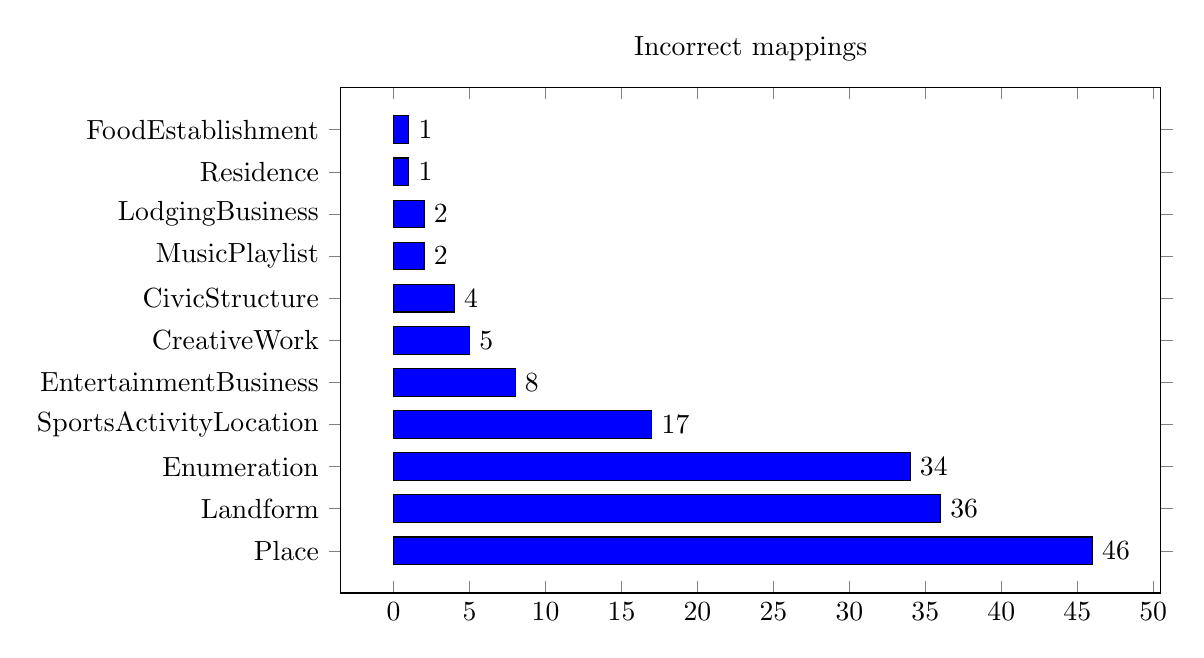
\begin{tikzpicture}
		\begin{axis}[
				title={Incorrect mappings},
				xbar,
				width=12cm, height=8cm,
				symbolic y coords={Place,Landform,Enumeration,SportsActivityLocation,EntertainmentBusiness,CreativeWork,CivicStructure,MusicPlaylist,LodgingBusiness,Residence,FoodEstablishment},
				ytick=data,
				nodes near coords, nodes near coords align={horizontal},
			]
			\addplot[fill=blue] coordinates {
				(46,Place)
				(36,Landform)
				(34,Enumeration)
				(17,SportsActivityLocation)
				(8,EntertainmentBusiness)
				(5,CreativeWork)
				(4,CivicStructure)
				(2,MusicPlaylist)
				(2,LodgingBusiness)
				(1,Residence)
				(1,FoodEstablishment)
			};
		\end{axis}
	\end{tikzpicture}
	\caption{Distribution of incorrect mappings in hypernym then siblings algorithm}
	\label{fig:incorrect}
\end{figure}

We picked the two most common incorrect mappings as objects of further study.
We went through all the cases of incorrect mapping to schema:Place.
This examination showed that in 45 of the 46 cases the mapping to schema:Place came as a result of
the synset being a hyponym of whole\#n\#2, which has the sibling geological\_formation\#n\#1 which again has a mapping to
schema:Landform, a sub type of schema:Place.
The last instance is the mapping from attention\#n\#3 which has the sibling tourist\_attraction\#n\#1 mapping to
schema:TouristAttraction.

For the mappings to schema:Landform all of the incorrect mappings came as a result of the synsets being hyponyms of part\#n\#3.
That synset has the hypernym thing\#n\#12 which has the hyponym body\_of\_water\#n\#1 which maps
to schema:BodyOfWater which again is a sub type of schema:Landscape.
Common for all these mappings is that the hypernyms are reasonable.
There is no reason to believe that these are cases where the hypernym chain breaks the semantics of the synset.
The mappings from WordNet to schema.org also seem to be sound.
This means that the source of the change in semantics must be looking at the siblings of the synset or its hypernyms.
There were instances of siblings both of the original synset and of the hypernyms,
so it does not appear that closeness to the synset needs to have any influence on whether or not the sibling gives
an accurate mapping for the synset.

\subsection{Choosing an algorithm}
From the previous discussion and from the results of the testing it seemed clear that the hypernyms first algorithm is
the dominant strategy for mapping synsets to schema.org, and that there is no difference between the two when mapping to SUMO.
The algorithms performed very differently when mapping to the different ontologies.

It might be that an increase in the number of mappings would change the results.
One could then try to refine the hypernym then siblings algorithm to analyse the mappings of its siblings,
and try to find some more sophisticated way of choosing which mapping to select.

It would also be interesting to try mapping to a more general ontology than schema.org.
As mentioned in section \ref{schemadotorg} schema.org is a small ontology with only 577 types,
and with a bias towards comercial interests.
It might be that an ontology that was larger,
and which had a more balanced approach to the world would result in better results for the algorithm.

As it stands it is clear that the hypernyms first algorithm out performed the hypernym then siblings algorithm,
and is the one that will be used in the artefact.
The fact that its mappings were incorrect or questionable in 6\% of the instances analyzed is unfortunate.
The cause of the errors were however found to be outside the system we have developed for this thesis,
and they have been reported.
This gives us reason to hope that the error rate of the system will go down as the tools it depends on are improved.
It also suggests that we should create some error reporting mechanism which we can use to give feedback to the maintainers
when incorrect mappings or hypernym relations occur.
%Noun list from http://www.desiquintans.com/articles.php?page=nounlist

%https://github.com/EivindEE/Master-thesis/blob/master/AlgComparison/AlgComparisonResultsBig
%https://github.com/EivindEE/Master-thesis/blob/master/AlgComparison/compare-different

\section{Testing against existing markup}
One of our success criteria was that it should be posible to mark up HTML as well or better than what is on the web now.
To test if we managed this we used pages that were allready marked up with schema.org markup,
and tried to generate similar markup using \theartefact\ before comparing the results to see if the metadata created
by the tool was of a similar quality.

\subsection{Method}
The method that we used to mark up and compare the sites followed a simple process.
Webpages were picked from a list of sites using the schema.org ontology for metadata which can be found on github
\footnote{\url{https://github.com/LawrenceWoodman/mida/wiki/Sites-Using-Microdata}}.

The markup of webpages that were picked were examined to find which things that were marked up,
and which schema.org types they were marked up as.
This process was selected to make sure we would be able to compare the results.

The pages were imported into the artefact, and the markup would be recreated by selecting text,
and if necessary supply keywords to disambiguate the content.
It was attempted to add the metadata as faithfully as possible to make comparison simpler
When the markup process was complete, the webpages would be exported and the resulting webpage would be analysed.
The original was used as a gold standard which the marked up pages could be compared to.

The analysis of the metadata would be performed by using Googles structured data testing tool
\footnote{\url{http://www.google.com/webmasters/tools/richsnippets}},
and W3s RDFa 1.1 distiller and parser\footnote{\url{http://www.w3.org/2012/pyRdfa/}}.
The structured data testing tool shows the metadata that is read and extracted by Google.
It was used to check if the metadata available to Google was the same.
The tool was used on both the original page and the page marked up by the artefact so that one could judge if the
extracted metadata was the same.
We could not use the RDFa distiller as it is created to distill RDFa, not microdata.
The RDFa distiller parses the webpage and extracts the RDFa, displaying it as some RDF format.
It was used to see that the markup that was created was valid RDFa and that it could be translated to RDF.

The pages we marked up using this process where:
\begin{itemize}
	\item A restaurant review from the Telegraph
	\item A tour operators customer feedback page
	\item A tourist agency home page
	\item The home page of a marketing company
	\item A movie review sites review of a film
\end{itemize}

The full HTML of the webpages before and after they were marked up using \theartefact\ can be found at
\url{https://github.com/EivindEE/Master-thesis/tree/master/WildTesting}.

Most of the metadata on the webpages that were marked up was metadata about larger sections of the page.
The most prevalent type used on the pages we marked up was schema:Review.
The artefact we developed is targeted towards disambiguating single words as described in section \ref{Interaction}.
When marking up the text this meant one had to decide whether to markup the same section of the text as used in the original page,
or if one should select a single word in the section describing its content.
Should one for example select the header review, or the entire review itself.
Choosing the first option would give the metadata a different structure,
while selecting the second option would require the user to provide a keyword describing the topic of the section.
Which of these strategies one chooses does not change the meaning of the metadata which is created by the tool.
A combination of these two strategies were used when marking up the pages.

\subsection{An issue with the testing tool}
An issue that was discovered when analyzing the resulting markup with the the structured data tool was that
it returned  error messages saying that some of the elements that had been marked up were missing required properties.
When analyzing a schema:Product without a name value the error message reads:

\begin{verbatim}
	Warning: Missing required field "name (fn)".
	Warning: Incomplete rdfa with schema.org.
\end{verbatim}

The documentation on the schema.org homepage does not give any indication that schema types have required properties.
The initial reaction to this was annoyance that these fields were required by RDFa but not by microdata.
Closer inspection of the unmodified webpages however revealed that when using the microdata format these types
were ignored without warning.
It is positive that the RDFa created by the artefact gives an error message instead of failing silently,
but it is not good that the testing tool describes a field as required when this is not mentioned in the documentation.
The fact that the validator requires the properties does not in it self mean that the markup is incorrect,
or that the syntax is wrong.
The validator is targeted towards the generation of rich snippets,
and it might be that the warning is intended to warn that the amount of metadata is insufficient to generate rich snippets.
The warning that required fields are missing might then refere to the fact that they are required to create a snippet,
not required for the metadata to be valid.
The metadata generated in these instances turned out to be of equal quality as that of the original documents,
but also showed that the tool could do more to promote attributes that are required by search engines.

\subsection{Comparison of the results}
We found that there are some schema.org types that we are not able to reach with the current system.
In particular we have found out the the system does not have a way to reach the aggregated schema.org types.
At the time of writing the aggregate types in schema.org are schema:AggregateRating and schema:AggregateOffer.
The type schema:AggregateRating is meant to represent the average rating that a rated object has received.
The type schema:AggregateOffer on the other hand represents a collection of offers for a given product.
The difficulty posed by both these types is that what separates them from their super types schema:Rating and schema:Offer
is that they represent the plurality of the super type.
The system uses WordNet to represent and disambiguate words, and as its basis for mapping natural language to ontologies.
WordNet is a dictionary type system, which does not separate between the different grammatical numbers of a given word,
as they all represent the same concept.
This could be an issue for the system as a whole since it means that the language we use as an intermediary between natural language
and the ontologies does not capture all of the complexity of the ontologies we wish to map to.
When these types were used in the documents they were instead mapped to their direct super type.

The exception we had to this was when the webpages used invalid types or properties in their metadata.
In the pages we checked we found one instance of invalid metadata.

Apart from this the results were found to be satisfactory,
and the tool was able to recreate all the metadata that was present on the original webpages.
In addition to being able to recreate all the metadata it also uncovered when the original used incorrect markup.
On the page with the movie review it was found that the author of the HTML had added an invalid property to a movie.
The webpage used the property name "publishdate" while the correct name of the property is "datePublished".
An advantage of using a tool like \theartefact\ is that one can be sure not to use incorrect properties such as this,
since the tool provides a list which only contain valid properties for the type one has selected.
These results show that the tool is able to create metadata of equal quality as that which is present on the web now.

\section{Browser rendering}
\label{Rendering}
One of the criteria for the artefact was that it should leave the visual representation of the system unchanged.
The system is meant to let users add metadata to existing webpages, and should not modify their appearance.
We did a comparison of the webpages before and after adding metadata.
You can see an example of the telegraph website before adding metadata in figure \ref{TelegraphOriginal},
and after in \ref{TelegraphData}.
We have cropped out the side margins and the header of the website in the images to make it easier to see the content of the sites.

\fig{TelegraphOriginal}{The Telegraph webpage before the metadata was added}
\fig{TelegraphData}{The Telegraph webpage with metadata added}

Looking at the figures we can see that the overall layout of the images is unchanged.
There are however some changes to the HTML.

To make the webpage appear the same when viewed on the URL the user is given when the page is exported
we replace relative URLs tied to images and \nom{CSS}{Cascading Style Sheets} with absolute URLs.
For simplicity we only change the URLs that start at the root of the domain.
So if there was an image on the page \texttt{http://example.org} which pointed to the source \texttt{/image.png}
then the source would be changed to \texttt{http://example.org/image.png}.
This change is not communicated to the user, which is unfortunate,
but it is posible to change if it leads to issues.

As one can see from the images there are some sections of the website which are not displayed, or more precisely they
are displayed as loading.
The switch from relative to absolute URLs have only been done for images and CSS,
which means that some of the javascript modules that the website depends on will not be loaded into the webpage.
We wanted to leave the HTML as much intact as possible,
and since the scripts have yet seemed crucial to display the page properly it was decided to leave them as they were.
It should be noted that this means that the page will sometimes miss some content, as visible in the figures.

One issue that might arrise is if some of the content on the site, either CSS or javascript,
depend on the order of the elements or their direct placement in the hierarchy.
Since \theartefact\ is intended to add metadata to user selected sections of the page we need to create our own
HTML elements to attach the metadata to, since that's the only reliable way to talk about just that section.
There are CSS selectors that select either direct children or the n-th children of an element.
Since we need to add elements it might be that the element we add cause another element to either not be the direct
child of the former parent, or that it changes the the elements number amongst the children.
In a similar way, DOM manipulation in javascript sometimes uses the children of an element or the index of an element
in a list of children.
We have not found any way to avoid this issue,
and can only hope that most developers depend on id and class attributes instead of the specific location in the DOM.

\section{Analysis of usage data}
In addition to the testing described earlier in this chapter we have also released the webapp on the internet.
This has allowed us to see how users who do not know the system would interact with it,
and if they could use it to add metadata.

The data we have at this point is inconclusive, but can hopefully give some indication of how the tool will be used.
The usage data we have collected contains the IP of the user.
We have used this information to exclude users from the UiB domain,
as this data would mostly consist of usage tied to testing or debugging the system in the development phase.
The usage data consists of the the data from the 8\textsuperscript{th}	 of April to the 12\textsuperscript{th} of May.

As mentioned, the tool is mainly targeted towards adding metadata to single words, with adding data to sections being
a secondary means of input.
This is consistent with how the users have used \theartefact.
From the usage data we have we can see that of the 298 of the text selections requests we have received,
only 12, or about 4\%, have been for selections so big that they have been categorized as sections of text.
The other 96\% of the selections were of single words or of single entities or concepts like "Alexander Graham Bell" or
"semantically classified lexical databases".

We have not found any cases of the users have used the resulting HTML on their webpages,
so it is not possible to say anything about their satisfaction with the page at this point.
